\documentclass{beamer}
\usetheme{Warsaw}
\usecolortheme{beaver}
\usepackage{graphicx}
\usepackage{circuitikz}
\usepackage{listings}
\usepackage{multirow}
\usepackage{multicol}



\lstset{language=verilog}

\title[Targetting Cell-Aware Faults]{\textsc{Intelligent Targeting of Cell-Aware-Faults by the use of mandatory conditions}}
\author[Micah A. Thornton]{\texorpdfstring{Micah A. Thornton\newline\url{mathornton@smu.edu}}{Micah A. Thornton} \\\vspace{0.2 em} \texorpdfstring{Fanchen Zhang\newline\url{fzhang@smu.edu}}{Fanchen Zhang} \\\vspace{0.2 em} \texorpdfstring{Jennifer Dworak\newline\url{jdworak@smu.edu}}{Jennifer Dworak}}
\institute{\textbf{Southern Methodist University \\Department of Computer Science and Engineering}}



\begin{document}
\begin{frame}
\maketitle
\end{frame}

\section{Introduction}
\begin{frame}{Outline}
\pause
\tableofcontents[pausesections]
\end{frame}

\frame{\tableofcontents[currentsection]}
\begin{frame}{Previous Work}
\begin{itemize}
    \item<2-> Cell-Aware Fault Model
    \begin{itemize}
    \item<3-> Proposed by Hapke et. al
    \item<4-> Models Analog Faults
    \item<5-> Difficult to do ATPG
    \item<6->Models faults as occurring within standard cells (logic gates)
    \item<7-> different from ``Cell-Aware-Type.'' (More on this to come)
    \end{itemize}
    \item<8-> Functional Simulation
    \begin{itemize}
    \item<9-> Used to Determine Fault Coverage (Shi `11)
    \item<10-> Overview valid state space
    \end{itemize}
    \item<11-> Extension of work on targeting very difficult stuck-at faults
\end{itemize}
\end{frame}

\subsection{Cell-Aware-Type Faults}
\begin{frame}{CAT Faults}
    \begin{itemize}
    \item<2-> Cell-Aware Type faults
    \begin{itemize}
    \item<3-> Discussed in Paper by Zhang et. al
    \item<4-> Model Cell-Aware Faults
    \item<5-> Use Stuck-At-ATPG to differentiate cell-aware-type faults.
    \end{itemize}
    \end{itemize}
    \pause\pause\pause\pause\pause
    \begin{block}{Note}
    \textit{This type of fault is considered different than a pure cell-aware fault because no Analog analysis is required to generate tests. This will be illustrated during the next example}
    \end{block}
\end{frame}

\subsection{Cell Aware Type Example}
\begin{frame}{CAT Example}
\pause
\begin{center}
imagine you have an inverter... 
\end{center}
\end{frame}

\begin{frame}{CAT Example}
\begin{center}
\begin{circuitikz}
\draw(0,0) node[not port] (not 1) {};
\end{circuitikz}
\end{center}
\end{frame}

\begin{frame}{CAT Example}
\begin{center}
\begin{circuitikz}
\draw
(2,1) node[pmos] (pmos) {}
(2,0) node[nmos] (nmos) {}
(0,0.5) node[] (Vin) {$V_{in}$}
(3,0.5) node[] (Vout) {$V_{out}$}
(2, -.5) node[ground] (gnd) {}
(Vin) -- (1,0.5)
(Vout) -- (2,0.5)
(nmos.G) -- (pmos.G)
(2,2) node[anchor=south] {$V_{dd}$};
\end{circuitikz}
\end{center}
\end{frame}

\begin{frame}{CAT Example}
\begin{center}
\begin{circuitikz}
\draw
(2,1) node[pmos] (pmos) {}
(2,0) node[nmos] (nmos) {}
(0,0.5) node[] (Vin) {$V_{in}$}
(3,0.5) node[] (Vout) {$V_{out}$}
(2, -.5) node[ground] (gnd) {}
(Vin) -- (1,0.5)
(Vout) -- (2,0.5)
(nmos.G) -- (pmos.G)
(2,2) node[anchor=south] {$V_{dd}$};
\end{circuitikz}
\begin{block}{Transistor Parameters}
$V_{tn} = V_{tp} = 0.7$ Volts. 
\end{block}
\end{center}
\end{frame}

\begin{frame}{CAT Example}
\begin{center}
But Transistors are not linear elements, so our model is still not perfect...
\end{center}
\end{frame}

\begin{frame}{CAT Example}
\begin{center}
During the manufacture of this inverter...
\end{center}
\end{frame}

\begin{frame}{CAT Example}
\begin{center}
\begin{circuitikz}
\draw
(2,1) node[pmos] (pmos) {}
(2,0) node[nmos] (nmos) {}
(0,0.5) node[] (Vin) {$V_{in}$}
(3,0.5) node[] (Vout) {$V_{out}$}
(2, -.5) node[ground] (gnd) {}
(Vin) -- (1,0.5)
(Vout) -- (2,0.5)
(nmos.G) -- (pmos.G)
(2,2) node[anchor=south] {$V_{dd}$}
(2,0.75) node[circ, color=red](ps){}
(2,1.25) node[circ, color=red](pd){};
\draw[color=red](ps) -- (pd)

;
\end{circuitikz}
\end{center}
\end{frame}

\begin{frame}{CAT Example}
\begin{center}
\begin{circuitikz}
\draw
(2,1) node[pmos] (pmos) {}
(2,0) node[nmos] (nmos) {}
(0,0.5) node[] (Vin) {$V_{in}$}
(3,0.5) node[] (Vout) {$V_{out}$}
(2, -.5) node[ground] (gnd) {}
(Vin) -- (1,0.5)
(Vout) -- (2,0.5)
(nmos.G) -- (pmos.G)
(2,2) node[anchor=south] {$V_{dd}$}
(2,0.75) node[circ, color=red](ps){}
(2,1.25) node[circ, color=red](pd){};
\draw[color=red](ps) -- (pd)

;
\end{circuitikz}\\
In this simple example cell... \\
\pause Set $V_{in}$ = 1, and observe $V_{out}$ = 1\\ 
\pause This analysis is difficult to perform on millions of transistors
\end{center}
\end{frame}

\subsection{}
\begin{frame}{CAT Example}
\begin{center}
With Cell-Aware-Type faults, we examine stuck-at ATPG test patterns... \\
\pause And add patterns that cause conflict, but might not be choosen by ATPG tool.
\end{center}
\end{frame}



\subsection{Functional Simulation}
\begin{frame}{Functional Simulation}
\begin{center}
Recall that the state space of an automaton refers to...
\\\pause All possible configurations of the memory elements in a device. \\ \pause Consider a general purpose device that contains fault F as shown: 
\end{center}
\end{frame}

\begin{frame}{Functional Simulation}
\begin{center}
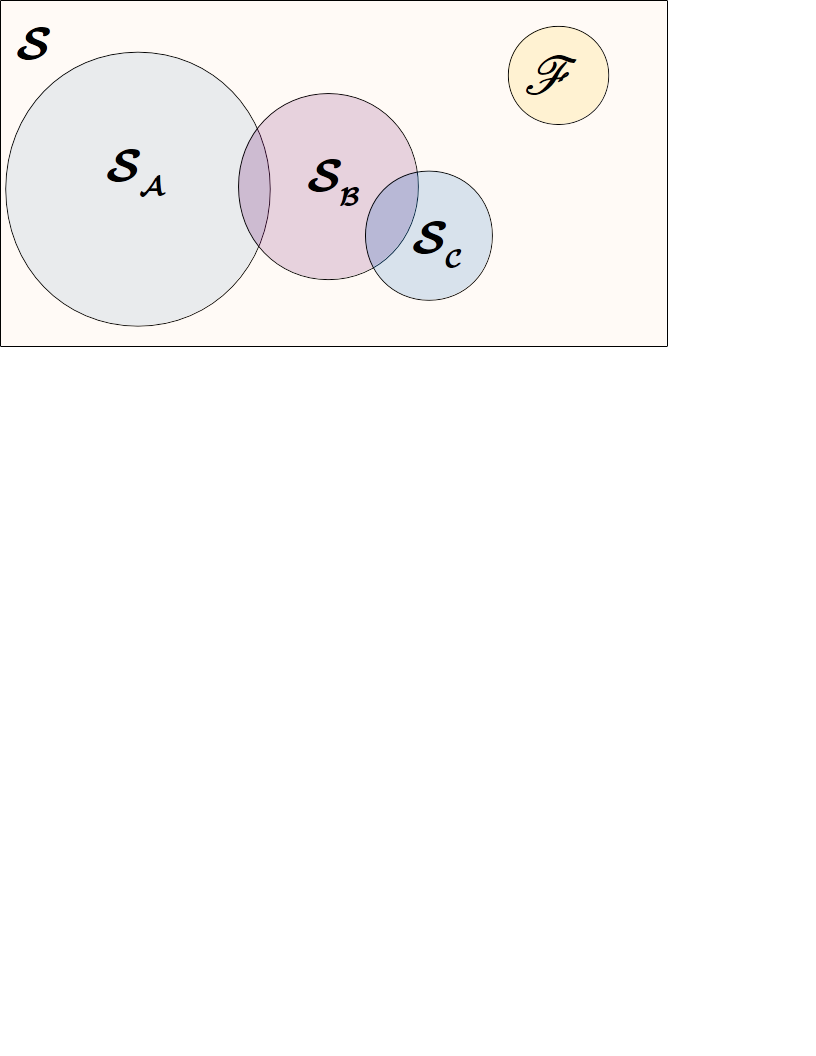
\includegraphics[scale=0.55]{Images/sd1.png}
\end{center}
\end{frame}

\begin{frame}{Functional Simulation}
\begin{center}
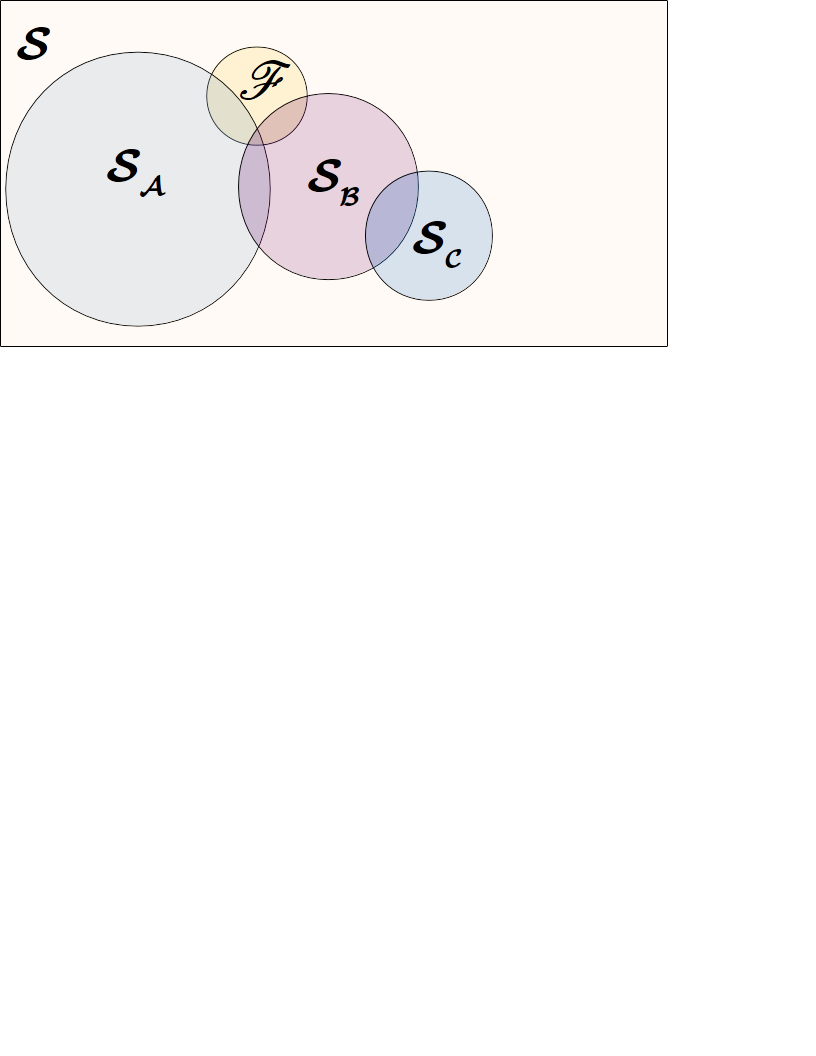
\includegraphics[scale=0.55]{Images/sd5.png}
\end{center}
\end{frame}

\begin{frame}{Functional Simulation}
\begin{center}
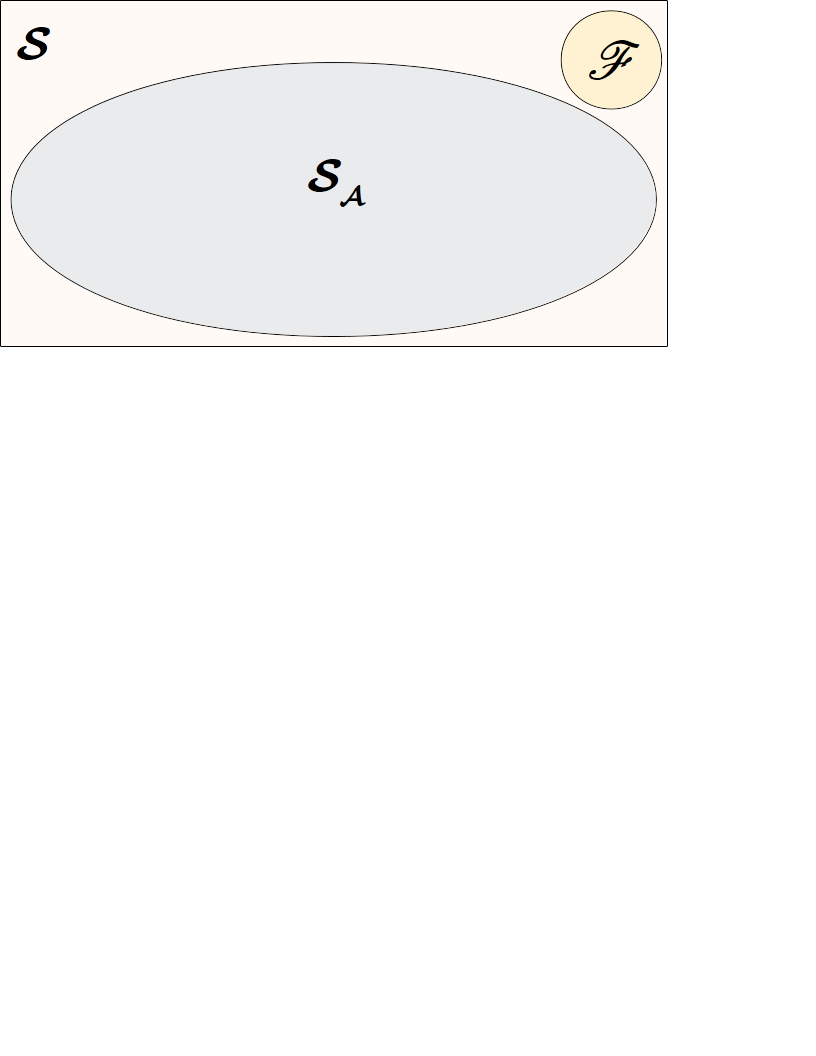
\includegraphics[scale=0.55]{Images/sd2.png}
\end{center}
\end{frame}

\begin{frame}{Functional Simulation}
\begin{center}
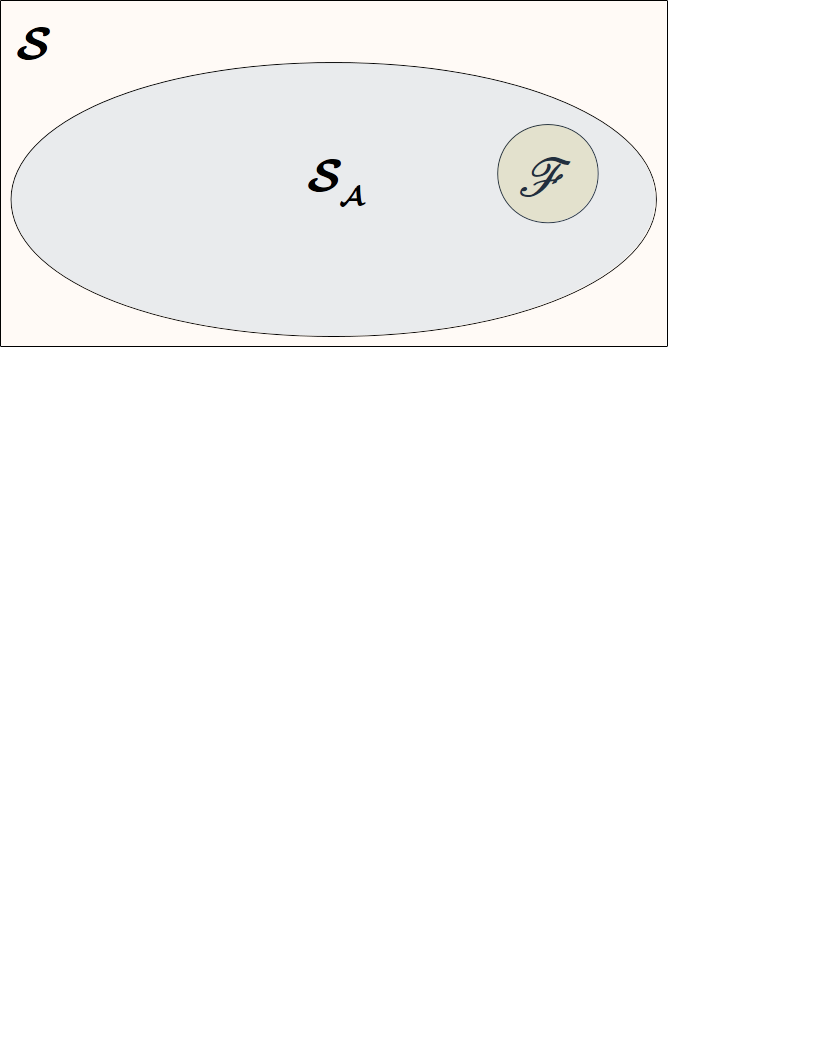
\includegraphics[scale=0.55]{Images/sd3.png}
\end{center}
\end{frame}

\begin{frame}{Functional Simulation}
\begin{center}
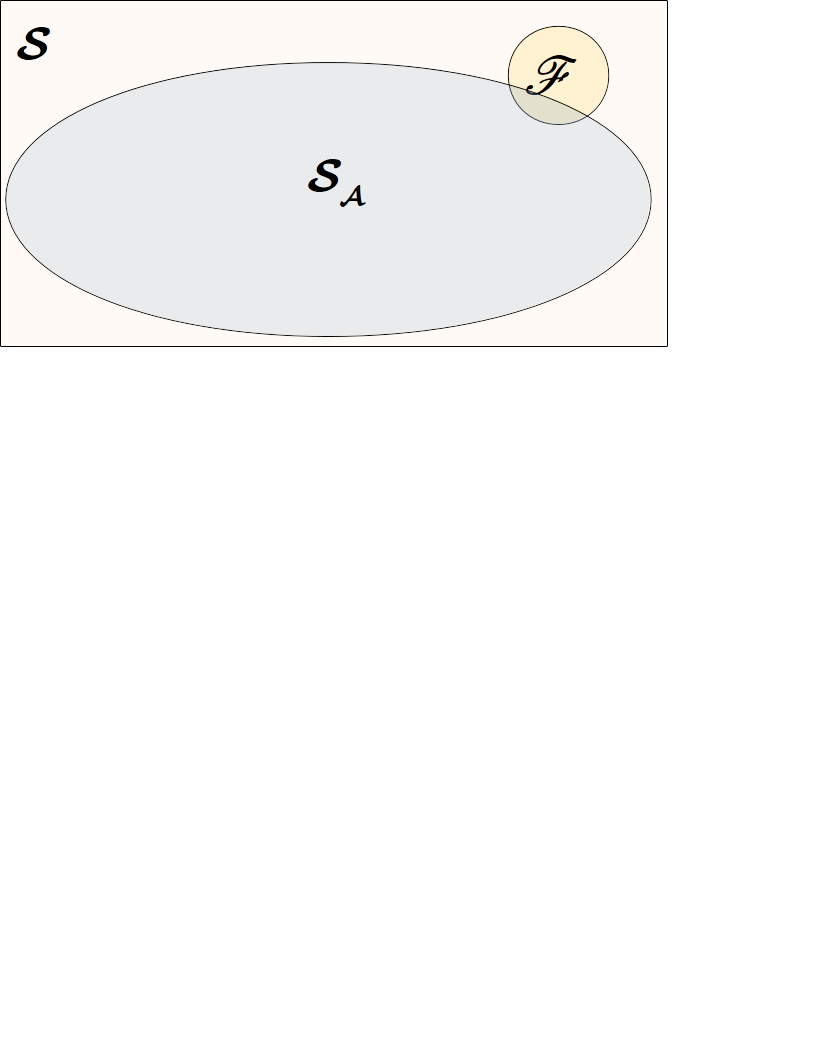
\includegraphics[scale=0.55]{Images/sd4.png}
\end{center}
\end{frame}

\subsection{Motivation}
\begin{frame}{CAT Example}
\begin{center}
ATPG for pure Cell-Aware Faults is Hard... \\
\pause It requires many resources (time/computational power) \\ 
\pause Let's prioritize faults using functional analysis of faults.
\end{center}
\end{frame}

\section{Experiment}
\frame{\tableofcontents[currentsection]}
\begin{frame}{Flow Chart}
\begin{center}
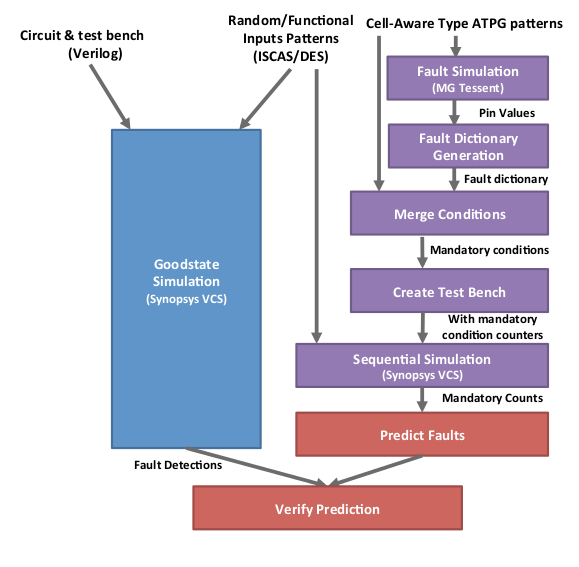
\includegraphics[scale = 0.3]{Images/flowDiagram.png}
\end{center}
\end{frame}

\begin{frame}[fragile]{Cell-Aware-Type UDFM Generation}
\lstset{breaklines=true, basicstyle=\ttfamily\scriptsize}\vspace{-1em}
\begin{lstlisting}[frame=single]

model s_faddx1_CO_(CO, CI, B, A)(
  model_source = verilog_udp;
  input (CI) ( )
  input (B) ( )
  input (A) ( )
  output (CO) (   )
  (
    primitive = _and mlc_sop_product_gate0 (B, A, mlc_product_net0_0);
    primitive = _and mlc_sop_product_gate1 (CI, A, mlc_product_net0_1);
    primitive = _and mlc_sop_product_gate2 (CI, B, mlc_product_net0_2);
    primitive = _or mlc_sop_sum_gate0 (mlc_product_net0_0, mlc_product_net0_1, mlc_product_net0_2, CO);
  ))
\end{lstlisting}

\end{frame}

\begin{frame}{Cell-Aware-Type UDFM Generation}
% \begin{center}
% \begin{circuitikz}
% \draw (0,4) node[american xor port] (xor1) {}
% (2,4) node[american xor port] (xor2) {}
% (2,2) node[american and port] (and1) {} 
% (2,0) node[american and port] (and2) {}
% (4,1) node[american or port] (or){}
% (xor1.in 1) node[anchor=east]{A}
% (xor1.in 2) node[anchor=east]{B}
% (and1.out) -- (or.in 1)
% (and2.out) -- (or.in 2)
% (xor2.in 2) -- (and1.in 1)
% (xor1.out) node[circ]{}
% (xor1.out) -- (and1.in 2)
% (xor1.in 1) node[circ] {}
% (xor1.in 2) node[circ] {}
% (xor1.in 1) -- (and2.in 1)
% (or.out) node[anchor=west]{$C_{out}$}
% (xor2.out) node[anchor=west]{S}
% (xor1.out) -- (xor2.in 1)
% (xor1.in 2) -- (and2.in 2)
% (0,3) node[anchor=east] (cin){}
% (and1.in 1) -- (cin); 
% \end{circuitikz}
% \end{center}

\begin{center}
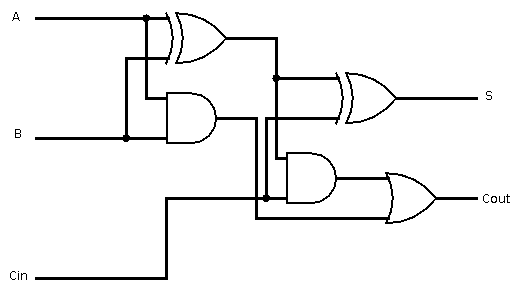
\includegraphics[scale=0.5]{Images/fulladder.png}
\end{center}
\end{frame}

\subsection{Cell-Aware-Type UDFM Generation}

\begin{frame}{Cell-Aware-Type UDFM Generation}
\begin{center}
\begin{table}
\begin{tabular} {c | c | c || c | c }
A & B & $C_{in}$ & $C_{out}$ & S\\
\hline
0&0&0&0&0 \\ 
0&0&1&0&1 \\
0&1&0&0&1 \\
0&1&1&1&0 \\
1&0&0&0&1 \\
1&0&1&1&0 \\
1&1&0&1&0 \\
1&1&1&1&1 \\

\end{tabular}
\end{table}
\end{center}
\end{frame}






\begin{frame}[fragile]{Cell-Aware-Type UDFM Generation}
\lstset{breaklines=true, basicstyle=\ttfamily\scriptsize}\vspace{-1em}
\begin{lstlisting}[frame=single]

        Cell ( "FADDX1" ) {
            Fault ( "FADDX1_i000_o1" ){
                Test {
                        StaticFault { "S" : 1; }
                        Conditions { "A" : 0; "B": 0; "CI": 0;}
                                }
                        }
            Fault ( "FADDX1_i000_o1" ) {
                Test {
                        StaticFault { "CO" : 1; }
                        Conditions { "A" : 0; "B": 0; "CI": 0;}
                                }
                        }
                }
\end{lstlisting}

\end{frame}

\subsection{Mandatory Condition Extraction}
\begin{frame}{Mandatory Condition Extraction}
\begin{center}
    Imagine you are testing a circuit with... \\
    \pause 6 Primary Inputs \\
    \pause 2 State Elements \\
    \pause you are looking for a fault $f$ \\
    \pause and perform stuck-at-ATPG 4 times (or with n=4 on n-detect)
    \end{center}
\end{frame}


\begin{frame}{Mandatory Condition Extraction}
    \begin{center}
    \vspace{-3 em}
    These were the patterns that detected it... \pause
    \vspace{2 em}
    \begin{tabular}{| c | c | c |}
        \hline
        & Inputs & Flip-Flops\\
        \hline
        \hline
        Pattern 1 & \textcolor{red}{0}1011\textcolor{red}{1} & 0\textcolor{red}{0} \\
        \hline
        Pattern 2 & \textcolor{red}{0}0100\textcolor{red}{1} & 1\textcolor{red}{0} \\
        \hline
        Pattern 3 & \textcolor{red}{0}1111\textcolor{red}{1} & 0\textcolor{red}{0} \\
        \hline
        Pattern 4 & \textcolor{red}{0}0000\textcolor{red}{1} & 1\textcolor{red}{0} \\
        \hline
    \end{tabular}
        \\\pause $MC(f) = \pause \overline{p_{0}}\pause p_{5}\pause \overline{d_{1}}$
        \end{center}
\end{frame}

\subsection{Circuit Goodstate Extraction Functional Simulation}
\begin{frame}{Circuit Goodstate Extraction Functional Simulation}
\begin{itemize}
    \pause
    \item This was reported on in the last publication.
    \pause
    \item we inserted scanchains into circuits (ISCAS/DES56)
    \pause
    \item Random inputs for ISCAS circuits
    \pause
    \item Functional Testbench patterns for DES (both encryption and decryption)
    \pause
    \item Captured state after every clock cycle, and had functional states for circuits.
\end{itemize}
\end{frame}


\subsection{Mandatory Counts During Functional Simulation}
\begin{frame}{Mandatory Counts During Functional Simulation}
\begin{itemize}
    \pause 
    \item After determining the mandatory conditions for each circuit
    \pause 
    \item Mandatory-Condition checking and gates were added to each circuit
    \pause 
    \item Using the goodstates we extracted 
    \pause
    \item We performed functional simulation on the circuit, 
    \pause 
    \item and counted the number of times the mandatory conditions occurred. 
    \end{itemize}
\end{frame}

\begin{frame}{MAND gates}
\begin{figure}[h!]
\centering
\caption{Mandatory Condition Detector for fault f\label{fig:mandgate}}
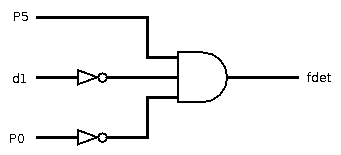
\includegraphics[scale=0.5]{Images/mand.png}
\end{figure} 
\end{frame}

\section{Results \& Analysis}
\frame{\tableofcontents[currentsection]}
\subsection{Mandatory Counts as Fault Classifiers}

\begin{frame}{ISCAS s9234}


\begin{figure}

\begin{center}
\begin{tabular}{cc|c|c|}
\cline{3-4}
& & \multicolumn{2}{ c| }{Detected} \\ \cline{3-4}
& & T & F\\ \cline{1-4}
\multicolumn{1}{ |c  }{\multirow{2}{*}{Predicted} } &
\multicolumn{1}{ |c| }{T} & 453 (TP) & 119 (FP)    \\ \cline{2-4}
\multicolumn{1}{ |c  }{}                        &
\multicolumn{1}{ |c| }{F} & 0 (FN) & 462 (TN)    \\ \cline{1-4}
\end{tabular}
\end{center}
\end{figure}

\begin{figure}
\vspace{1 em}
\begin{center}
\begin{tabular}{| c | c |}
\hline
Statistic &  Value \\
\hline
\hline
Precision & 79\% \\ 
\hline 
Accuracy & 88\% \\ 
\hline 
Specificity & 79\% \\ 
\hline 
Fall-out & 20.5\% \\ 
\hline
\end{tabular}
\end{center}
\end{figure}


\end{frame}

\begin{frame}{DES 56}
\begin{figure}[h!]
\vspace{1 em}
\begin{center}
\begin{tabular}{cc|c|c|}
\cline{3-4}
& & \multicolumn{2}{ c| }{Detected} \\ \cline{3-4}
& & T & F\\ \cline{1-4}
\multicolumn{1}{ |c  }{\multirow{2}{*}{Predicted} } &
\multicolumn{1}{ |c| }{T} & 461 (TP) & 2 (FP)    \\ \cline{2-4}
\multicolumn{1}{ |c  }{}                        &
\multicolumn{1}{ |c| }{F} & 0 (FN) & 14 (TN)    \\ \cline{1-4}
\end{tabular}
\end{center}
\end{figure}
\begin{figure}[h!]
\vspace{1 em}
\begin{center}
\begin{tabular}{| c | c |}
\hline
Statistic &  Value \\
\hline
\hline
Sensitivity & 100\% \\ 
\hline
Accuracy & 99.5\% \\ 
\hline
Specificity & 87.5\% \\ 
\hline
Fall-out & 14.2\% \\ 
\hline
Precision & 99.5\% \\
\hline
\end{tabular}
\end{center}
\end{figure}
\end{frame}

\subsection{Regression Analysis}

\begin{frame}{ISCAS s9234}
\begin{center}
    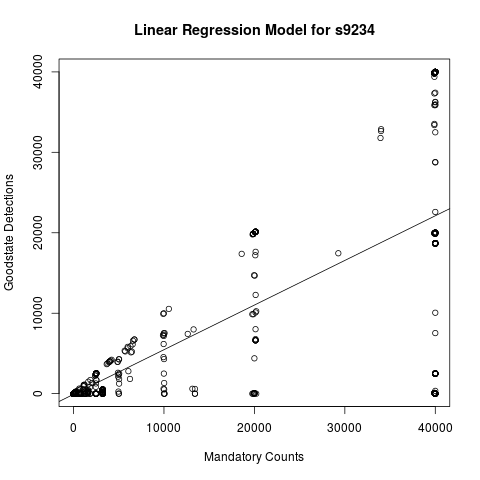
\includegraphics[scale=0.40]{Images/s9234linereg.png}
\end{center}
\end{frame}

\begin{frame}{DES 56}
\begin{center}
    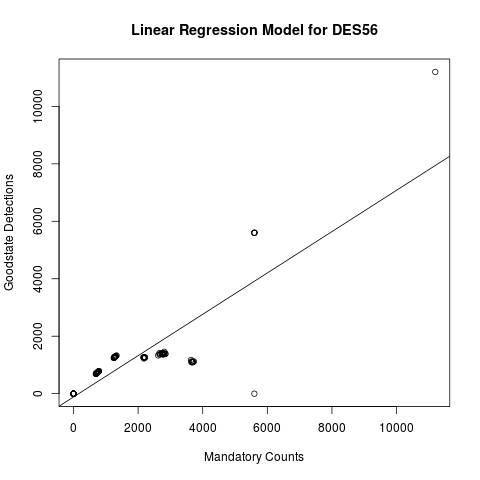
\includegraphics[scale=0.40]{Images/deslinereg.png}
\end{center}
\end{frame}
\section{Conclusion}
\frame{\tableofcontents[currentsection]}
\begin{frame}{Conclusion}
\begin{itemize}
\pause
    \item Cell-Aware fault model describes faults within cells
    \pause
    \item Large number of C.A. Faults for given circuits
    \pause
    \item Functional Simulation and Mandatory Conditions allow us to prioritize fault detections
    \pause
    \item We provided examples of mandatory condition calculations, and showed how they could be used to predict whether or not a cell-aware fault is functional
\end{itemize}
\end{frame}

\section{Acknowledgement}
\frame{\tableofcontents[currentsection]}
\begin{frame}{Acknowledgement}

\begin{center}
The authors would like to thank Semiconductor Research Corporation who supports this research under Task ID 2465.001. The authors are also grateful for the support of our industrial liaisons. \\ 
\vspace{2em}
\textbf{Thank You}
\end{center}
\end{frame}

\begin{frame}{}
\begin{center}\Huge{\textsc{Questions?}}\end{center}
\end{frame}

\end{document}